\clearpage
\addappheadtotoc
\appendixpage

\appendix


\section{Solución problemas Ubuntu Server }
\subsection{Problema RAID 1 al desconectar un disco.}
Cuando sacamos por pimera vez un disco del RAID, el dispositivo md se desactiva, para solucionar esto deberemos seguir los siguientes pasos:
En primer lugar iniciamos la maquina virtual y llegara un momento en el que ponga ``waiting for encrypted source device'' (Figura \ref{fig10}) una vez ahí, debemos esperar unos 3 minutos hasta que aparece el promt de initframfs.
Una vez llegados a este punto ejecutamos la orden: \texttt{ cat /proc/mdstat } y podremos ver que el RAID esta desactivado, para solucionarlo ejecutaremos la orden \texttt{mdadm -R /dev/md0}, una vez hecho esto ejecutaremos \texttt{exit} para salir de initramfs y la maquina virtual comenzará a arrancar con normalidad ( Figura \ref{fig11}). \cite{manmdadm}

Tras esto debemos recordar que debemos añadir un nuevo disco al RAID (\texttt{ mdadm /dev/mdX -a /dev/sdXX}) para que vuelva a estar completo.

\begin{figure}[H]
    \begin{center}
        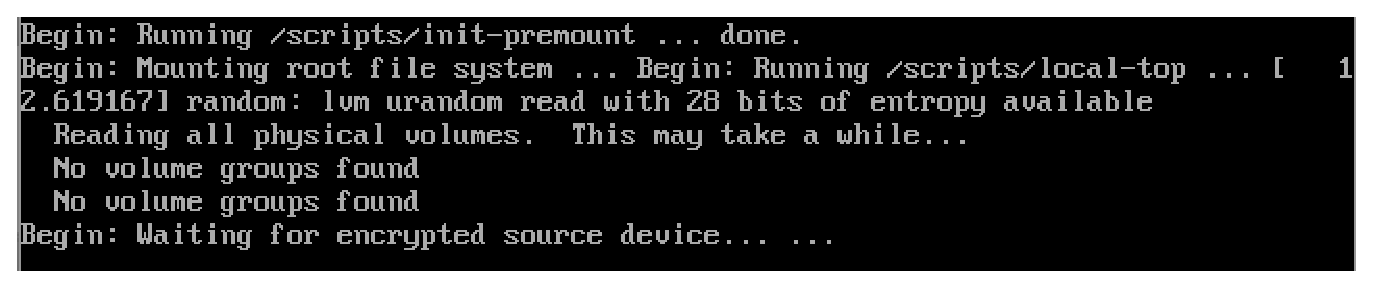
\includegraphics[scale=0.6]{Imagenes/waiting}
        \caption{Mensaje:``waiting for encrypted source device''.}
        \label{fig10}
    \end{center}
\end{figure}

\begin{figure}[H]
    \begin{center}
        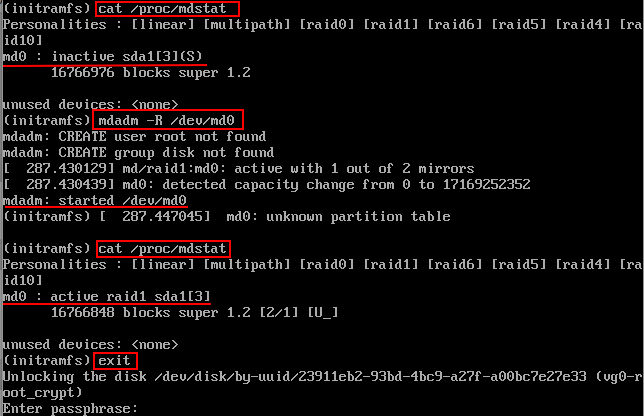
\includegraphics[scale=0.5]{Imagenes/activar}
        \caption{Proceso para arreglar el RAID.}
        \label{fig11}
    \end{center}
\end{figure}


\label{praid}
\subsection{error:  Diskfilter writes are not supported}
Este error es un bug de Ubuntu, que se puede solucionar con el procefimiento indicado en: \href{http://askubuntu.com/questions/468466/why-this-occurs-error-diskfilter-writes-are-not-supported/468487#468487}{boot - Why this occurs error: Diskfilter writes are not supported - Ask Ubuntu}
